
%(BEGIN_QUESTION)
% Copyright 2009, Tony R. Kuphaldt, released under the Creative Commons Attribution License (v 1.0)
% This means you may do almost anything with this work of mine, so long as you give me proper credit

Determine all actions that will result in an {\it increased} product temperature in the ``hot product'' pipe (as it exits the heat exchanger), assuming the use of saturated steam (i.e. steam at its boiling/condensing temperature) as the heating fluid:

$$\includegraphics[width=15.5cm]{i00015x01.eps}$$

Identify the validity of each possible action in this list by checking boxes in the table -- whether the action will result in an increased product temperature or whether it will not.  Assume all valves are throttling (neither fully open nor fully closed, but each one working to restrict flow through it), and that the words ``open'' and ``close'' refer to incremental motion rather than extreme travel (i.e. opening or closing each valve just a bit, rather than {\it fully} opening or {\it fully} closing each valve):

% No blank lines allowed between lines of an \halign structure!
% I use comments (%) instead, so that TeX doesn't choke.

$$\vbox{\offinterlineskip
\halign{\strut
\vrule \quad\hfil # \ \hfil & 
\vrule \quad\hfil # \ \hfil & 
\vrule \quad\hfil # \ \hfil \vrule \cr
\noalign{\hrule}
%
% First row
{\bf Action} & {\bf Will work} & {\bf Will not work} \cr
%
\noalign{\hrule}
%
% Another row
Open valve A &  & \cr
%
\noalign{\hrule}
%
% Another row
Close valve A &  & \cr
%
\noalign{\hrule}
%
% Another row
Open valve B &  & \cr
%
\noalign{\hrule}
%
% Another row
Close valve B &  & \cr
%
\noalign{\hrule}
%
% Another row
Increase steam supply pressure &  & \cr
%
\noalign{\hrule}
%
% Another row
Decrease steam supply pressure &  & \cr
%
\noalign{\hrule}
%
% Another row
Increase incoming feed temperature &  & \cr
%
\noalign{\hrule}
%
% Another row
Open valve C &  & \cr
%
\noalign{\hrule}
%
% Another row
Close valve C &  & \cr
%
\noalign{\hrule}
} % End of \halign 
}$$ % End of \vbox


\vfil 

\underbar{file i00015}
\eject
%(END_QUESTION)





%(BEGIN_ANSWER)

This is a graded question -- no answers or hints given!

%(END_ANSWER)





%(BEGIN_NOTES)

An important principle concerning any heat exchanger may be stated as follows: {\it if fluid ``A'' heats fluid ``B'', then fluid ``B'' cools fluid ``A''.}  In this particular example, steam is used as the heating medium for some unspecified product fluid.  Thus, steam is heating the product, while the product is cooling the steam.

\vskip 10pt

Any change in steam flow rate with a given product flow rate will directly affect product effluent temperature, and also directly affect condensate temperature.   The direct influence of steam flow on the temperature of the exiting product is rather simple to see: more or less hot steam input to the exchanger directly affects the amount of heat added to the product, and therefore the product's final temperature.  The direct influence of steam flow on condensate temperature is easiest to see from the perspective of cooling: the flow rate of steam inversely affects the amount of {\it time} each steam molecule spends inside the exchanger getting cooled off by the product.

\vskip 10pt

Any change in product flow rate with a given steam flow rate will inversely affect product effluent temperature, and also inversely affect condensate temperature.  The inverse influence of product flow on exiting product temperature is based on the time each product molecule spends inside the exchanger being heated by the steam.  The inverse influence of product flow on condensate temperature is based on the change in cooling effect that the product has on the steam.


% No blank lines allowed between lines of an \halign structure!
% I use comments (%) instead, so that TeX doesn't choke.

$$\vbox{\offinterlineskip
\halign{\strut
\vrule \quad\hfil # \ \hfil & 
\vrule \quad\hfil # \ \hfil & 
\vrule \quad\hfil # \ \hfil \vrule \cr
\noalign{\hrule}
%
% First row
{\bf Action} & {\bf Will work} & {\bf Will not work} \cr
%
\noalign{\hrule}
%
% Another row
Open valve A &  & $\surd$ \cr
%
\noalign{\hrule}
%
% Another row
Close valve A & $\surd$  & \cr
%
\noalign{\hrule}
%
% Another row
Open valve B &  & $\surd$ \cr
%
\noalign{\hrule}
%
% Another row
Close valve B & $\surd$  & \cr
%
\noalign{\hrule}
%
% Another row
Increase steam supply pressure & $\surd$  & \cr
%
\noalign{\hrule}
%
% Another row
Decrease steam supply pressure &  & $\surd$ \cr
%
\noalign{\hrule}
%
% Another row
Increase incoming feed temperature & $\surd$  & \cr
%
\noalign{\hrule}
%
% Another row
Open valve C & $\surd$  & \cr
%
\noalign{\hrule}
%
% Another row
Close valve C &  & $\surd$ \cr
%
\noalign{\hrule}
} % End of \halign 
}$$ % End of \vbox


%INDEX% Physics, temperature: heat exchangers
%INDEX% Process: heat exchanger temperature/flow control (generic)

%(END_NOTES)


